\section{Tổng quan}

\begin{frame}[shrink=10]{Bối cảnh}
    \begin{block}{Bối cảnh}
    Trong nhiều bài toán học máy, dữ liệu đầu vào thường có số chiều rất lớn:
    mỗi mẫu được mô tả bởi rất nhiều biến số, đặc trưng hoặc tín hiệu đo đạc.
    \end{block}

    \vspace{0.2cm}
    \small
    \begin{columns}[T]
        \begin{column}{0.49\textwidth}
            \textbf{Ví dụ điển hình}
            \begin{itemize}
                \item Ảnh số có hàng trăm đến hàng nghìn pixel hoặc đặc trưng.
                \item Dữ liệu y sinh chứa nhiều chỉ số định lượng.
                \item Dữ liệu cảm biến và hành vi có nhiều biến theo thời gian.
                \item Dữ liệu văn bản có không gian đặc trưng rất lớn.
            \end{itemize}
        \end{column}
        \begin{column}{0.49\textwidth}
            \textbf{Ba khó khăn chính}
            \begin{itemize}
                \item Khoảng cách giữa các điểm dữ liệu trở nên kém trực quan và kém phân biệt.
                \item Mô hình có nhiều tham số hơn, dễ quá khớp.
                \item Chi phí tính toán và lưu trữ tăng mạnh.
            \end{itemize}
        \end{column}
    \end{columns}

    \vspace{0.15cm}
    \smallskip
    \textbf{Tóm lại:} hiện tượng này thường được gọi là \textbf{curse of dimensionality}.
\end{frame}

\begin{frame}{Đặt vấn đề}
    Từ bối cảnh trên, bài thuyết trình xoay quanh ba câu hỏi:

    \vspace{0.15cm}
    \begin{enumerate}
        \item Có thể rút gọn dữ liệu về không gian thấp chiều hơn mà vẫn giữ lại thông tin quan trọng hay không?
        \item Nếu dữ liệu có thể được phân tách gần tuyến tính, liệu các mô hình đơn giản có đủ hiệu quả không?
        \item Nếu cấu trúc dữ liệu hoặc biên quyết định là phi tuyến, ta cần mở rộng mô hình như thế nào?
    \end{enumerate}

    \vspace{0.15cm}
    \begin{block}{Kết luận}
        Ba câu hỏi này dẫn trực tiếp tới ba nhóm phương pháp:
        \textbf{Dimension Reduction}, \textbf{Linear Classification} và
        \textbf{Non-linear Learning Algorithms}.
    \end{block}
\end{frame}

\begin{frame}[shrink=3]{Mapping ba chủ đề trong pipeline học máy}
    \renewcommand{\arraystretch}{1.2}
    \footnotesize
    \begin{tabular}{p{0.2\linewidth} p{0.21\linewidth} p{0.22\linewidth} p{0.25\linewidth}}
        \toprule
        \textbf{Chủ đề} & \textbf{Vai trò} & \textbf{Đầu ra chính} & \textbf{Câu hỏi trọng tâm} \\
        \midrule
        Dimension Reduction & Nén thông tin, trực quan hóa, khử nhiễu & Biểu diễn thấp chiều $z \in \mathbb{R}^K$ & Dữ liệu thực sự sống trong không gian nào? \\
        \addlinespace
        Linear Classification & Dự đoán nhãn bằng siêu phẳng & Nhãn dự đoán hoặc xác suất lớp & Có thể tách lớp bằng một ranh giới tuyến tính không? \\
        \addlinespace
        Non-linear Learning Algorithms & Mô hình hóa biên quyết định phức tạp & Quy tắc quyết định phi tuyến & Nếu siêu phẳng không đủ, cần mô hình mạnh hơn nào? \\
        \bottomrule
    \end{tabular}

    \vspace{0.15cm}

    \begin{block}{Tóm lại}
    \textbf{\textcolor{blue}{Giảm chiều dữ liệu}} giúp xây dựng một biểu diễn gọn và hiệu quả hơn, 
    tạo nền tảng cho các bước học máy tiếp theo. Trên cơ sở đó, 
    \textbf{\textcolor{blue}{các mô hình phân loại tuyến tính}} đóng vai trò như một cách tiếp cận đơn giản, 
    dễ diễn giải và thường hiệu quả khi dữ liệu gần tuyến tính. 
    Trong những trường hợp cấu trúc dữ liệu phức tạp hơn, 
    các \textbf{\textcolor{blue}{phương pháp học phi tuyến}} được sử dụng để mở rộng khả năng biểu diễn của mô hình.
    \end{block}
    \hfill{\scriptsize Nguồn chính: \cite{duchesnay2021statsml}}
\end{frame}

\begin{frame}{Pipeline}
    \begin{figure}
    \centering
    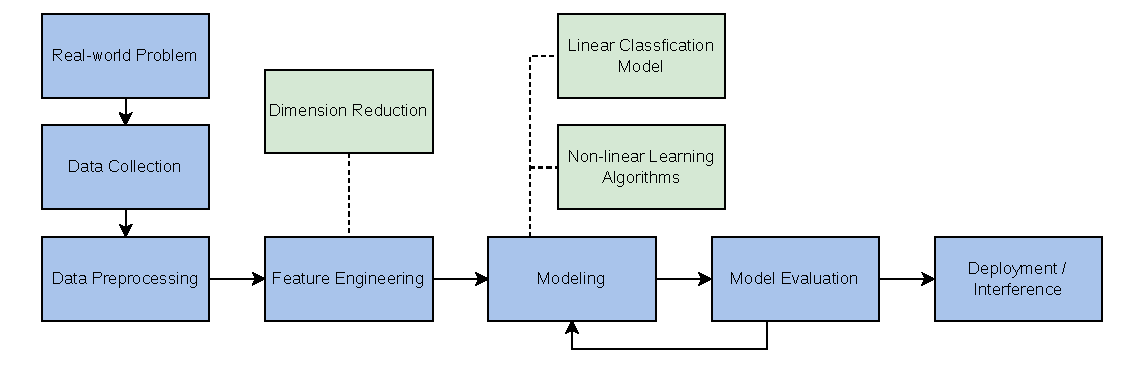
\includegraphics[width=1.0\textwidth]{img/pipeline.pdf}
    \caption{Pipeline Machine Learning và vị trí các phương pháp}
    \end{figure}
\end{frame}


